\subsection{PMT Voltage Dividers}

In the original readout electronics for CLAS, the single output from each PMT was amplified by a factor of 10 and then
split in two to feed the ADC and TDC boards. This amplification and splitting was performed by a dedicated electronic
module (UVA 132)~\cite{Adams:2001kk}. This unit was replaced by a pulse amplifier board entirely powered by the
current flowing through the base voltage divider. This board was developed in 2002 at Jefferson Lab
\cite{Popov:2003mj}. The new electronics provided a factor of 10 PMT signal boost, while preserving the fast PMT
pulse shape. It also significantly improved the signal amplitude and the signal to noise ratio: the high voltage needed
to detect the single photoelectron signal (SPE) was reduced on average by 374~V, see \F{pmtHVImprovement}.

\begin{figure}[H]
	\centering
	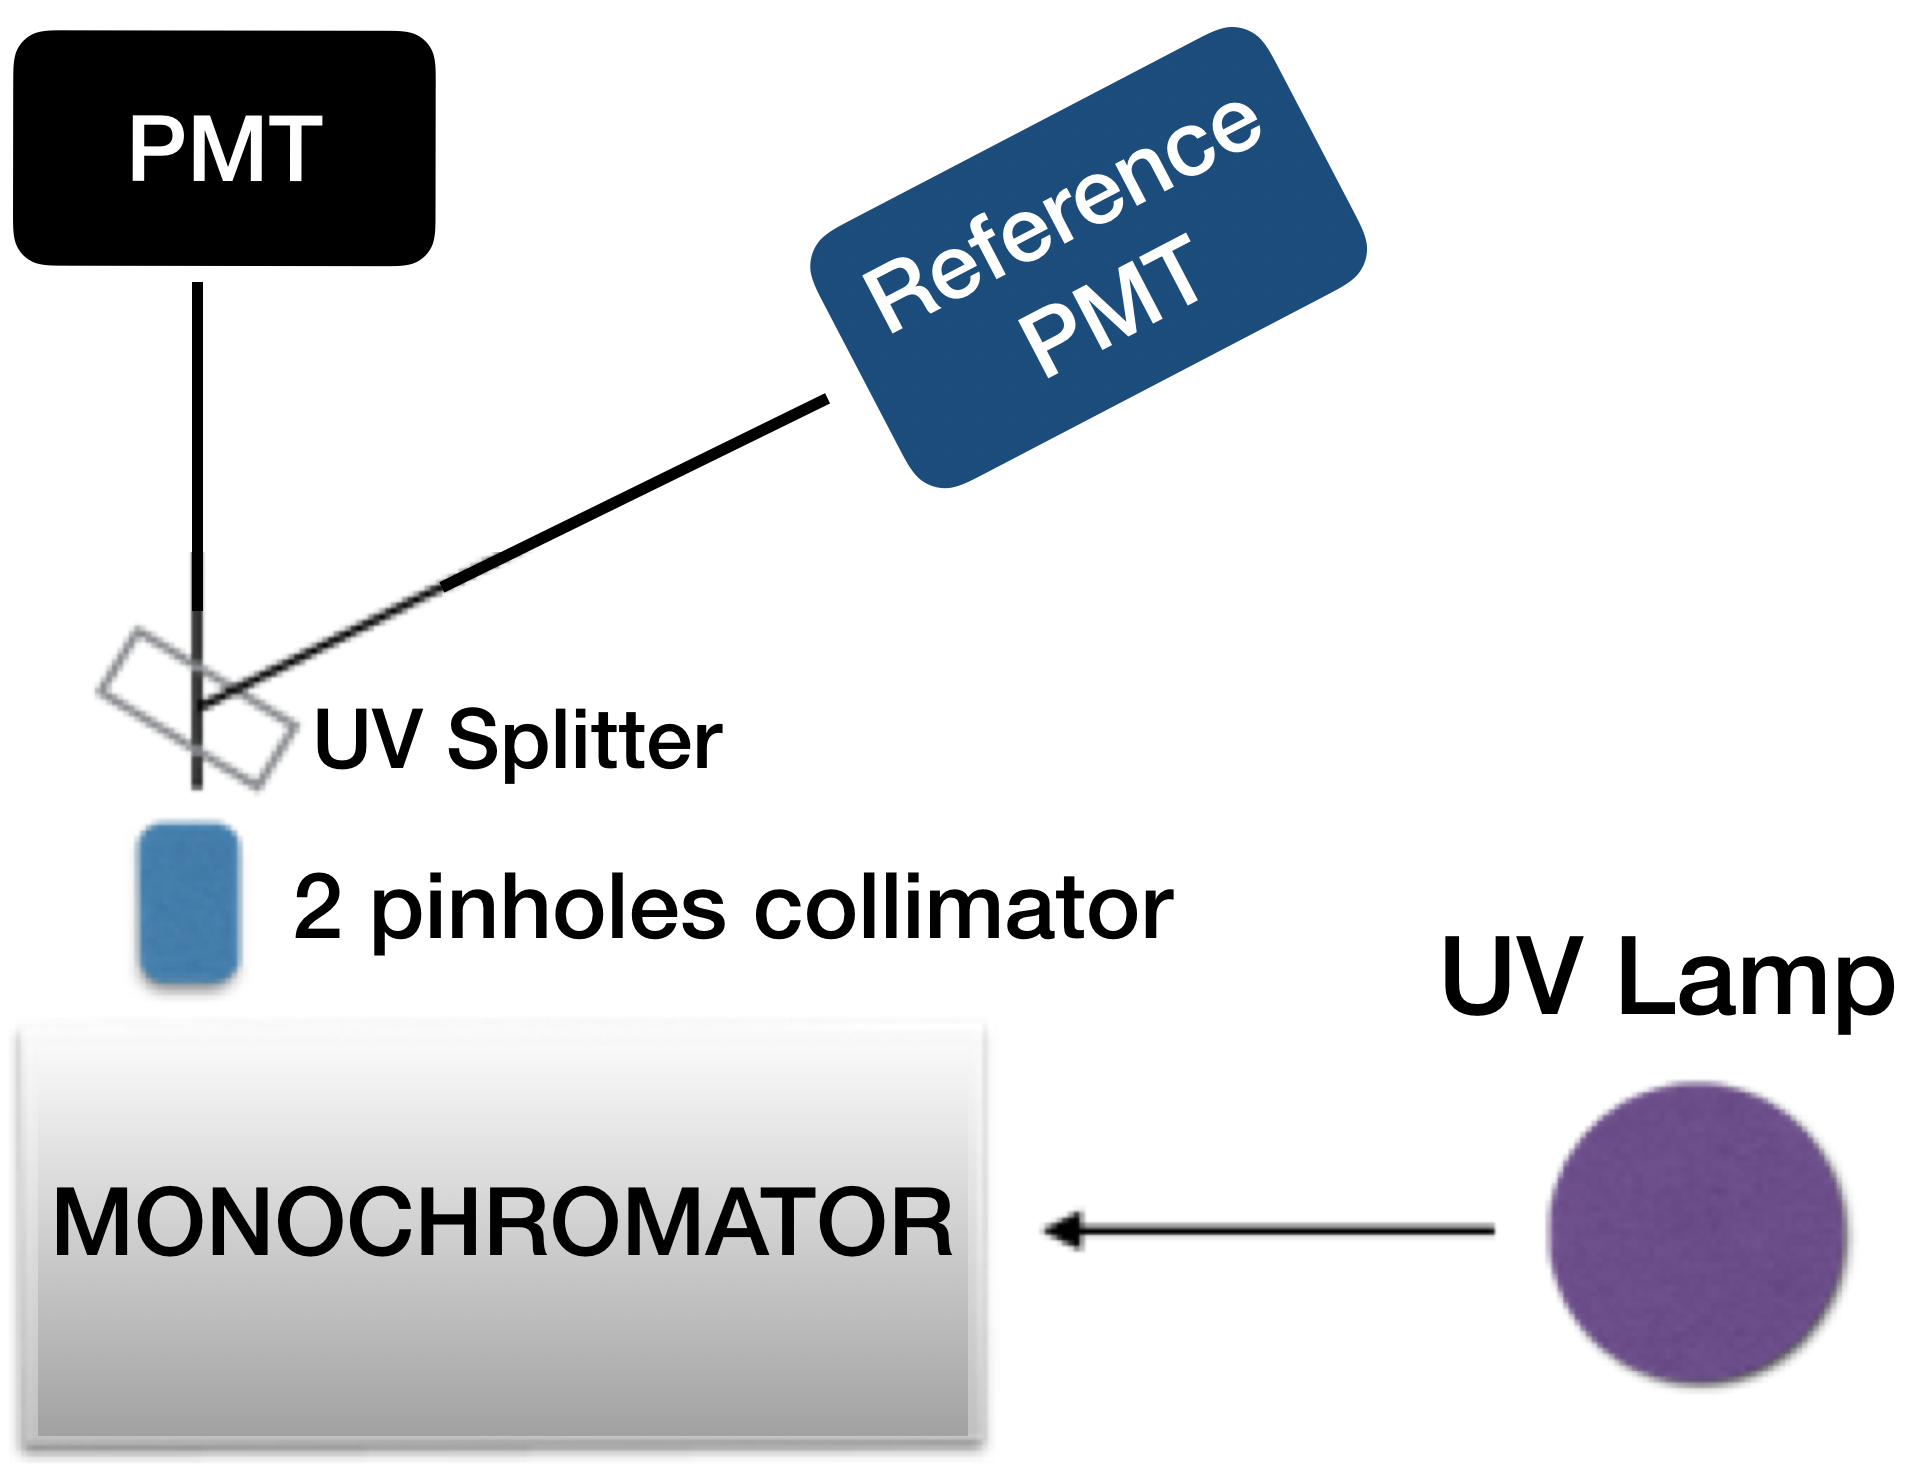
\includegraphics[width=0.99\columnwidth, height=0.65\columnwidth]{img/pmtTestingSetup.png}
	
\includegraphics[width=0.99\columnwidth, keepaspectratio]{img/blank.png}
	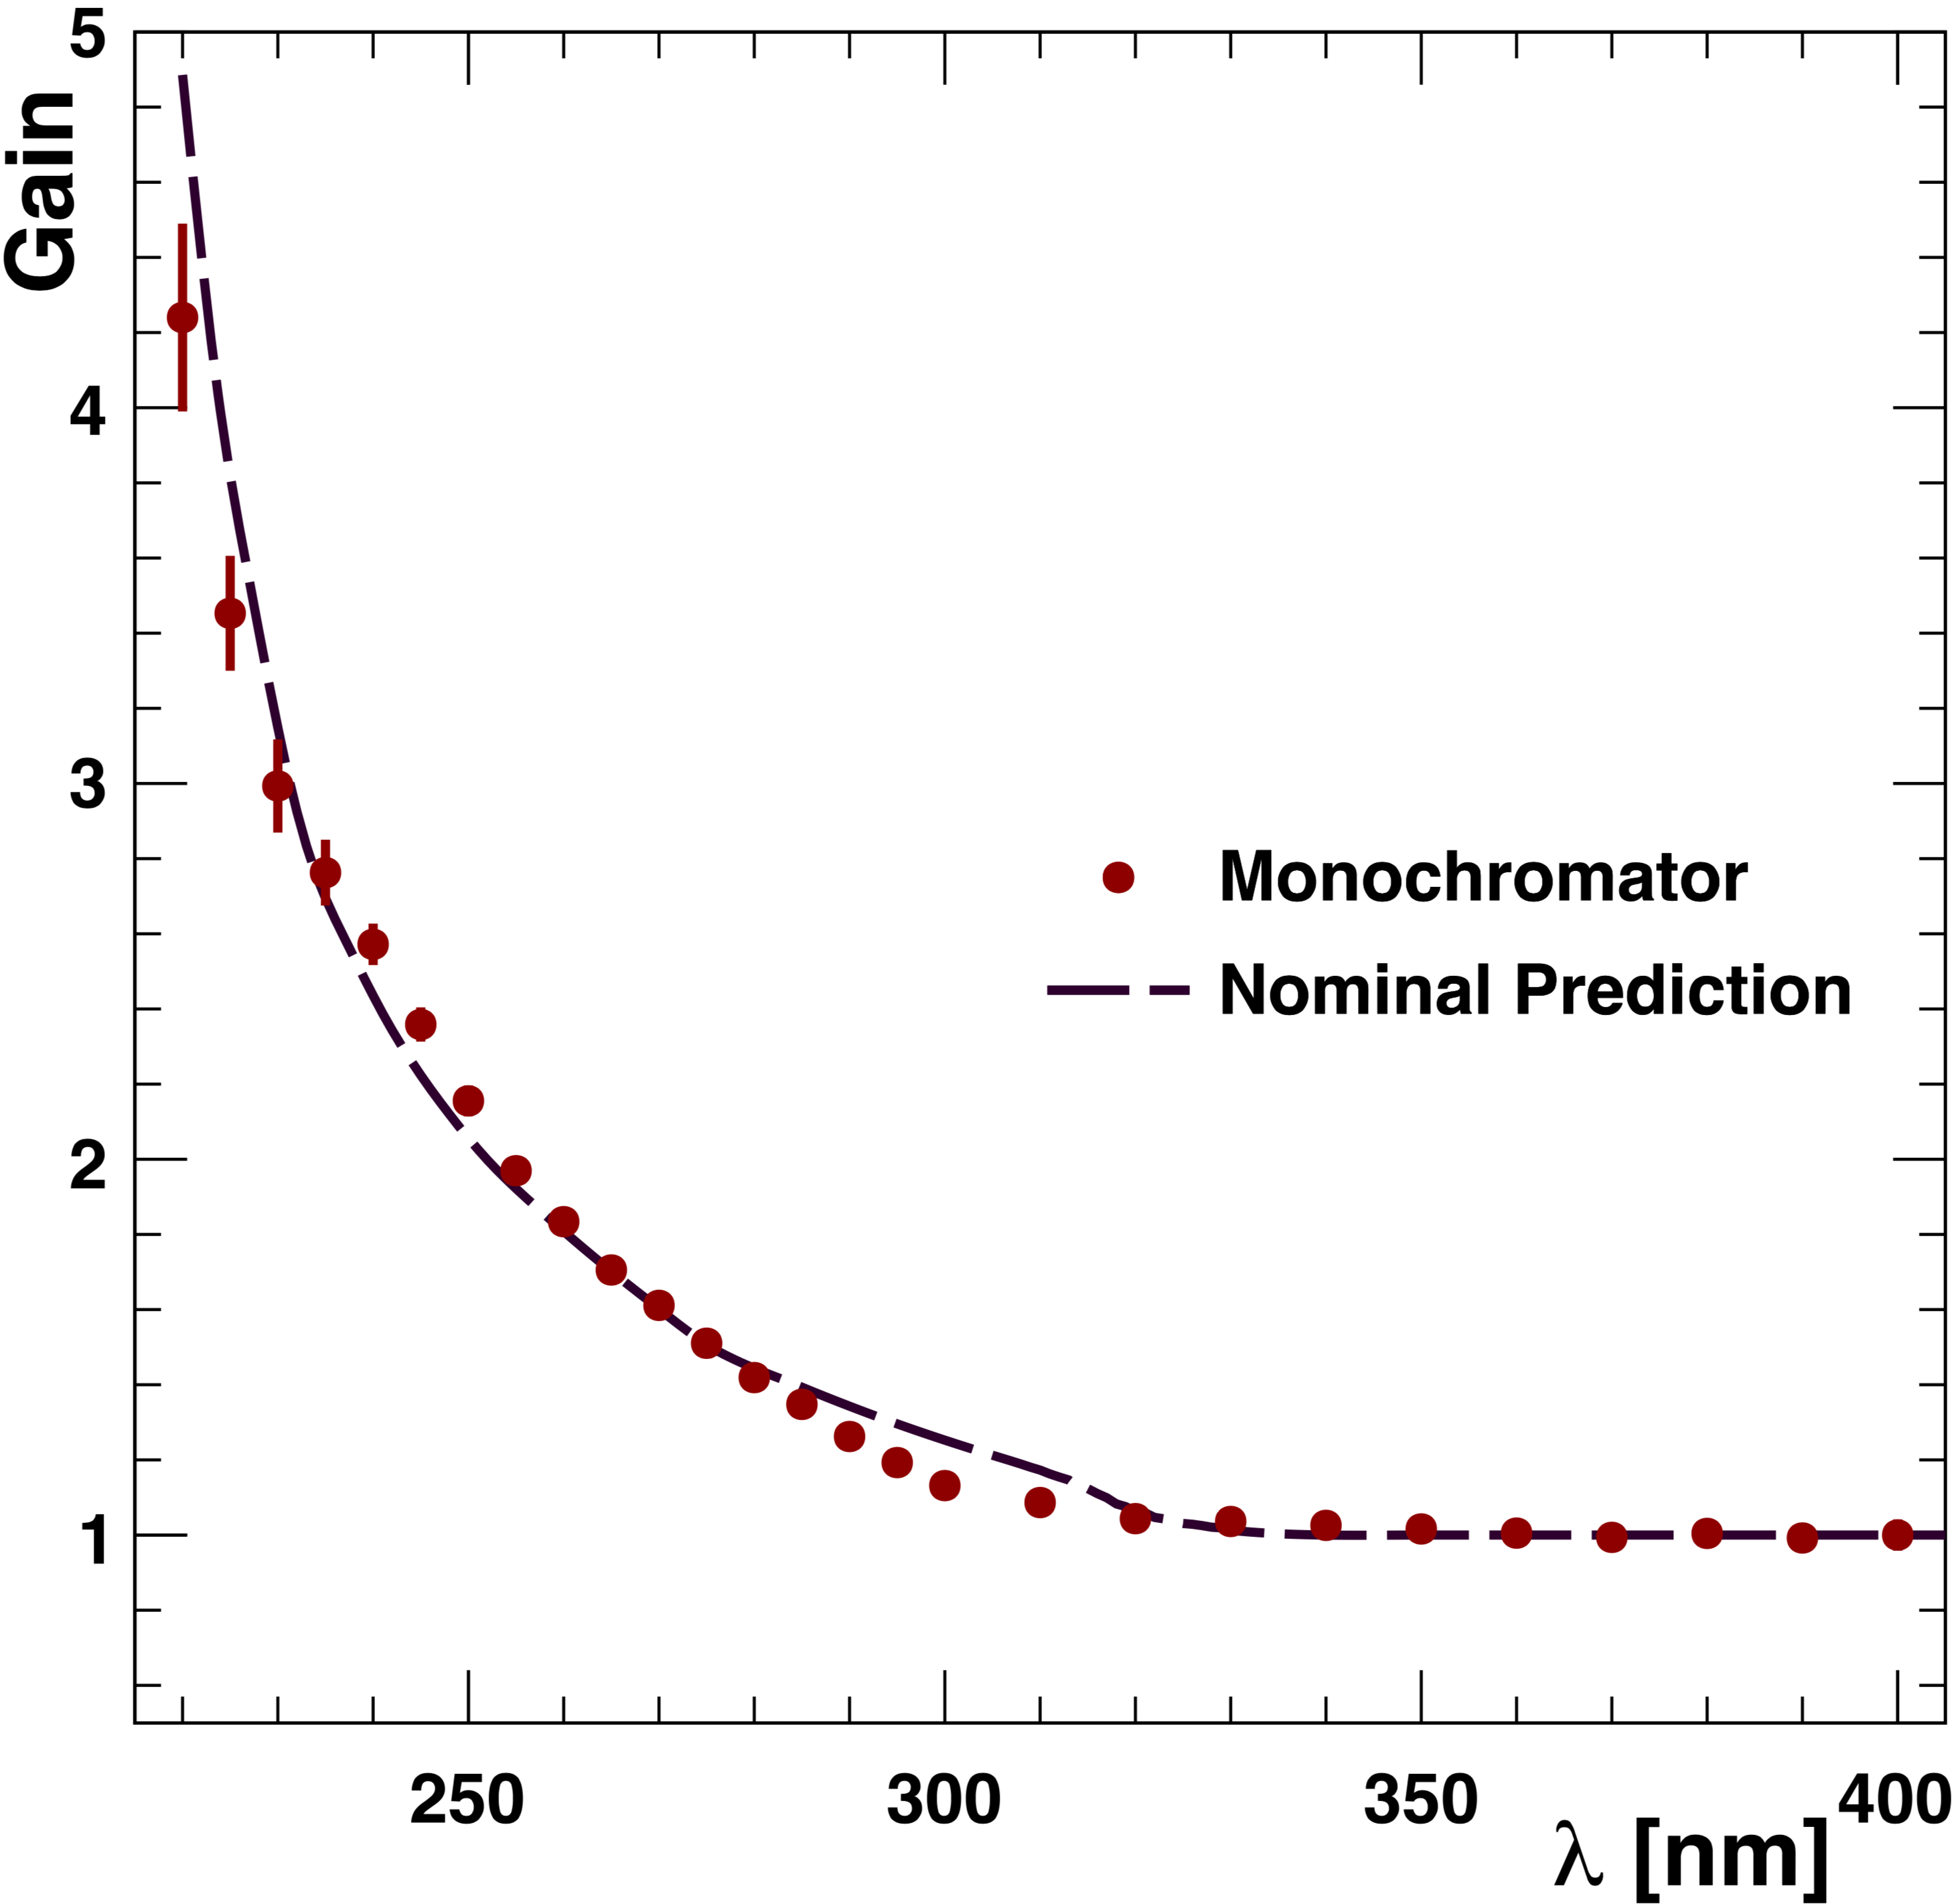
\includegraphics[width=0.99\columnwidth, keepaspectratio]{img/ptQEResults.png}
	\caption{Top: Monochromator setup used for the gain measurements. Bottom: Results from the monochromator
          measurements (red circles), compared to the nominal prediction for a p-terphenyl material load of
          110~$\mu$g/cm$^2$ (dashed line).}
	\label{fig:pmtTestingSetupAndptQEResults}
\end{figure}

The amplifier board design was adapted to use the LTCC XP4500B base and a prototype, shown in \F{pmtWithDivider}, was
built to provide a factor of ten amplification and a split signal directly from the PMT base.

\begin{figure}
	\centering
	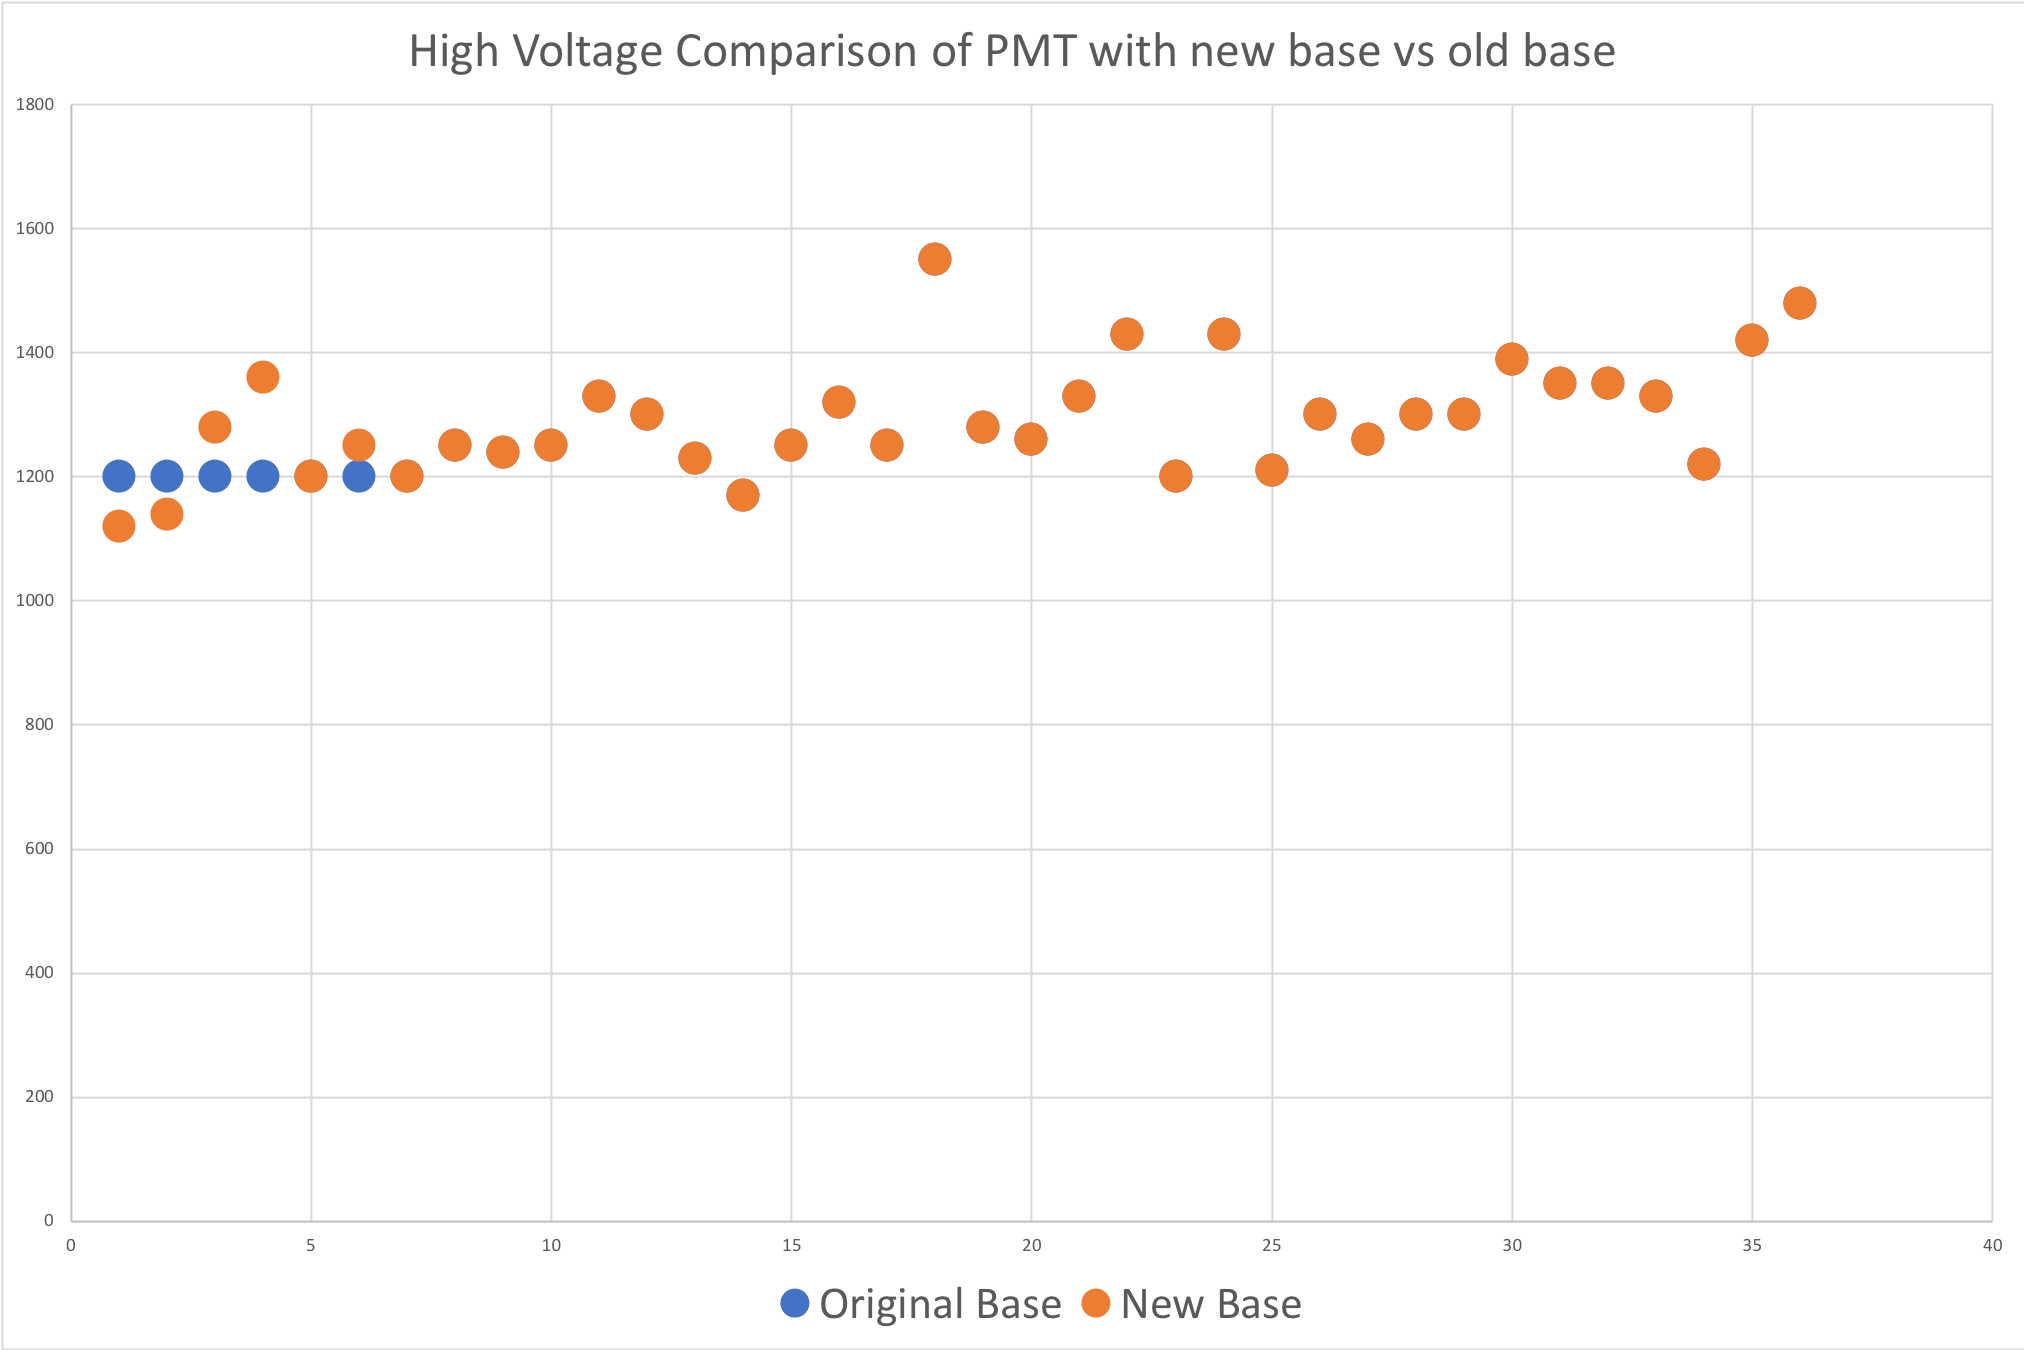
\includegraphics[width=0.99\columnwidth,keepaspectratio]{img/pmtHVImprovement.png}
	\caption{Comparison of the 36 PMT high voltages (in V) in one LTCC box gain-matched to provide a SPE peak at about
          ADC channel 200. The PMTs with the modified bases produce the same response function as the original base but at
          an average voltage 374~V less (1666~V vs. 1292~V).}
	\label{fig:pmtHVImprovement}
\end{figure}


\begin{figure*}[!ht]
	\centering
	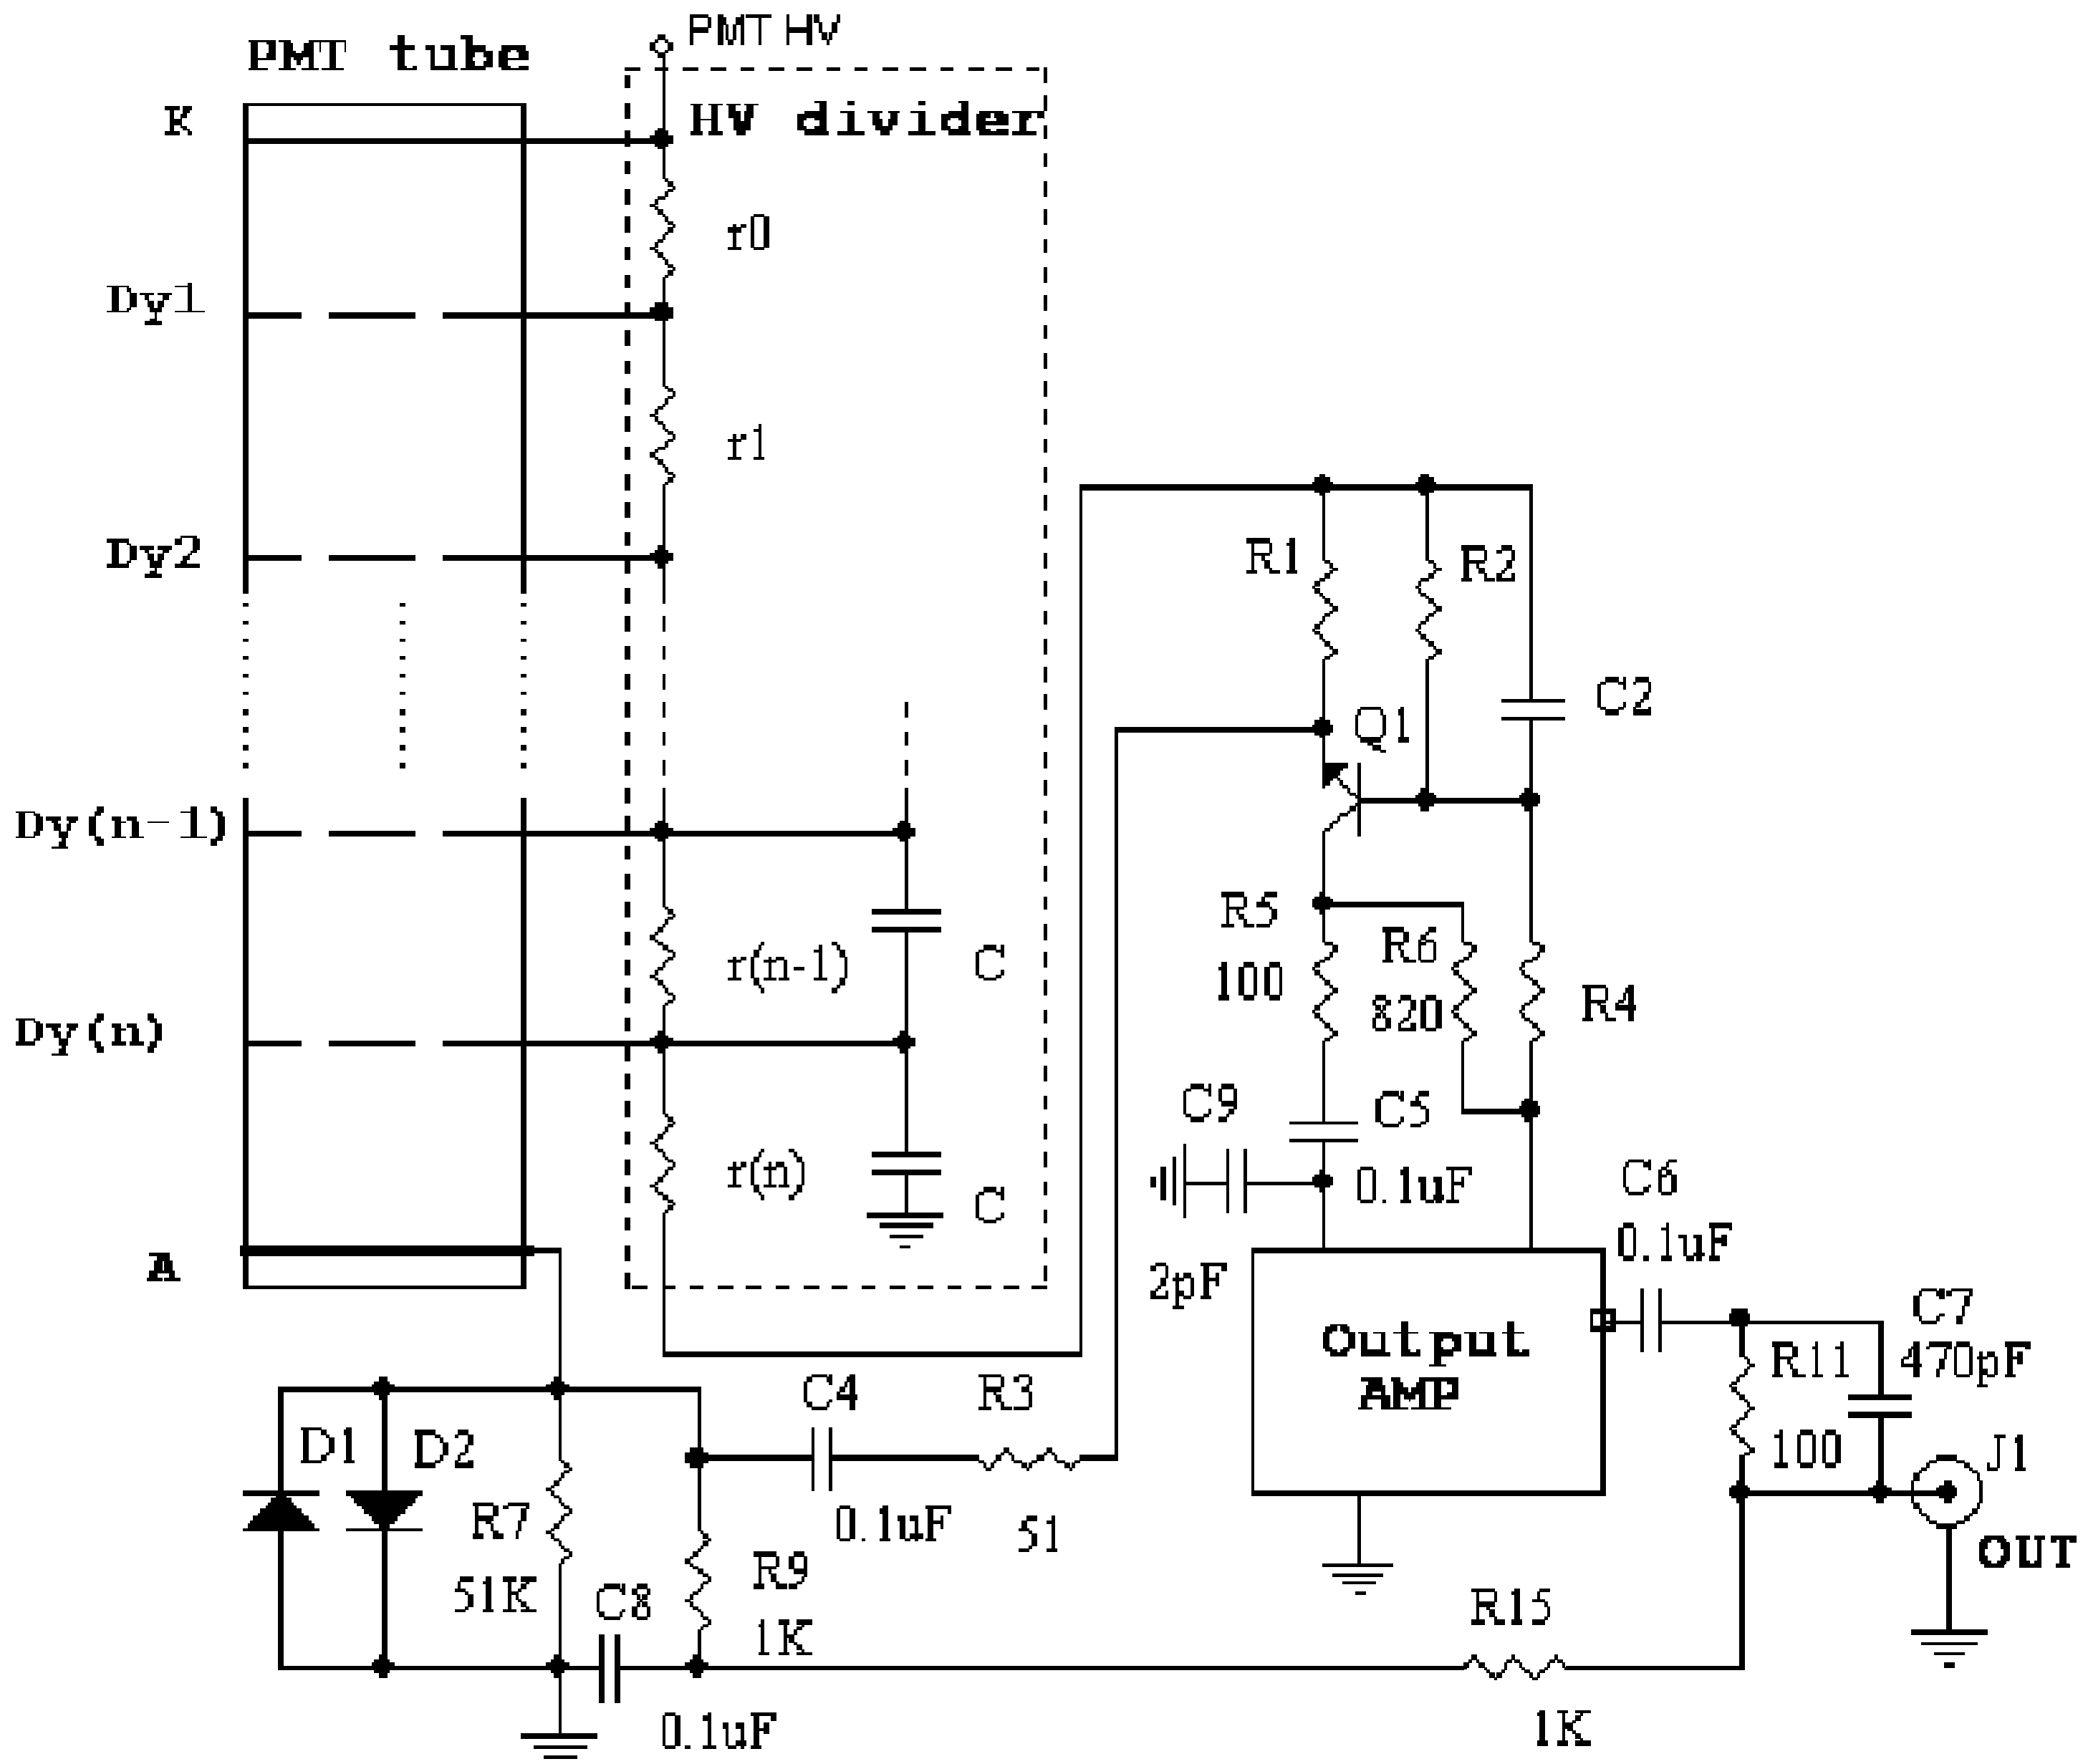
\includegraphics[width=1.25\columnwidth, keepaspectratio]{img/dividerSchematic.png}
	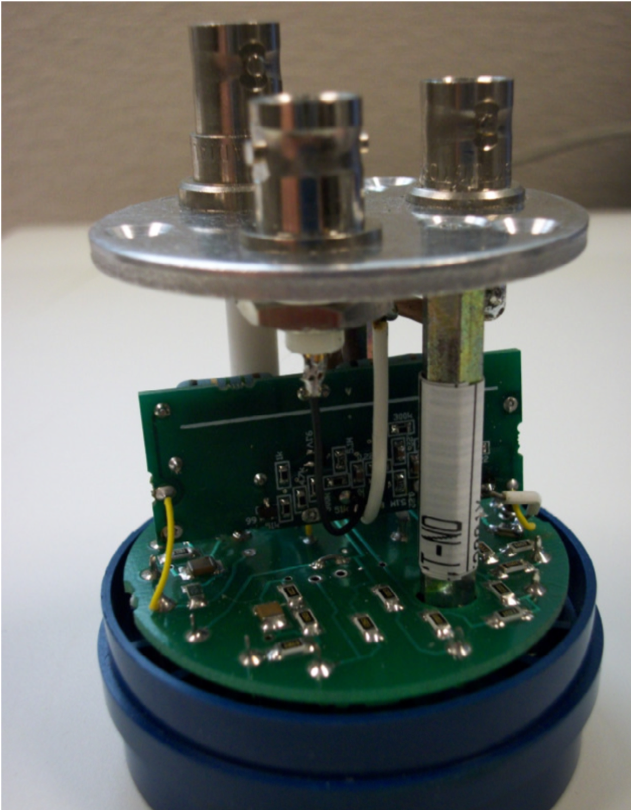
\includegraphics[width=0.75\columnwidth, height=0.95\columnwidth]{img/pmtWithDivider.png}
	\caption{Left: schematic of the PMT amplifier board, shown as a resistor chain for simplicity. The amplifier, designed
          to operate at currents from 0.7 to 1.5~mA, provides amplification in the first stage using a common base amplifier,
          made of a fast NPN transistor NE68033 by California Eastern Laboratories. In the output stage a PNP-NPN transistor
          is used. Right: the prototype module installed in the XP4500B PMT base. The bottom of the base has been modified to
          contain the HV SHV input and two output signals.}
	\label{fig:pmtWithDivider}
\end{figure*}

In \F{dividerTests} a comparison of the two signals shows the similarity between the two outputs. During testing of the
modified PMT bases, the output was processed by a flash ADC (FADC) read out by a data acquisition system using the PMT
itself as the trigger. The corresponding SPE spectrum was analyzed. The shape of the SPE signal is very similar to the
original signal coming from the external dedicated splitter and amplifier through the ADC electronics shown in
\F{dividerTests} (right).

180 bases were assembled at Jefferson Lab and installed on the PMT dividers. Both signals from all of the modified
bases were tested. The response of the PMTs, amplified by a factor of 10, was verified to be identical to the original
output.

\begin{figure}
	\centering
	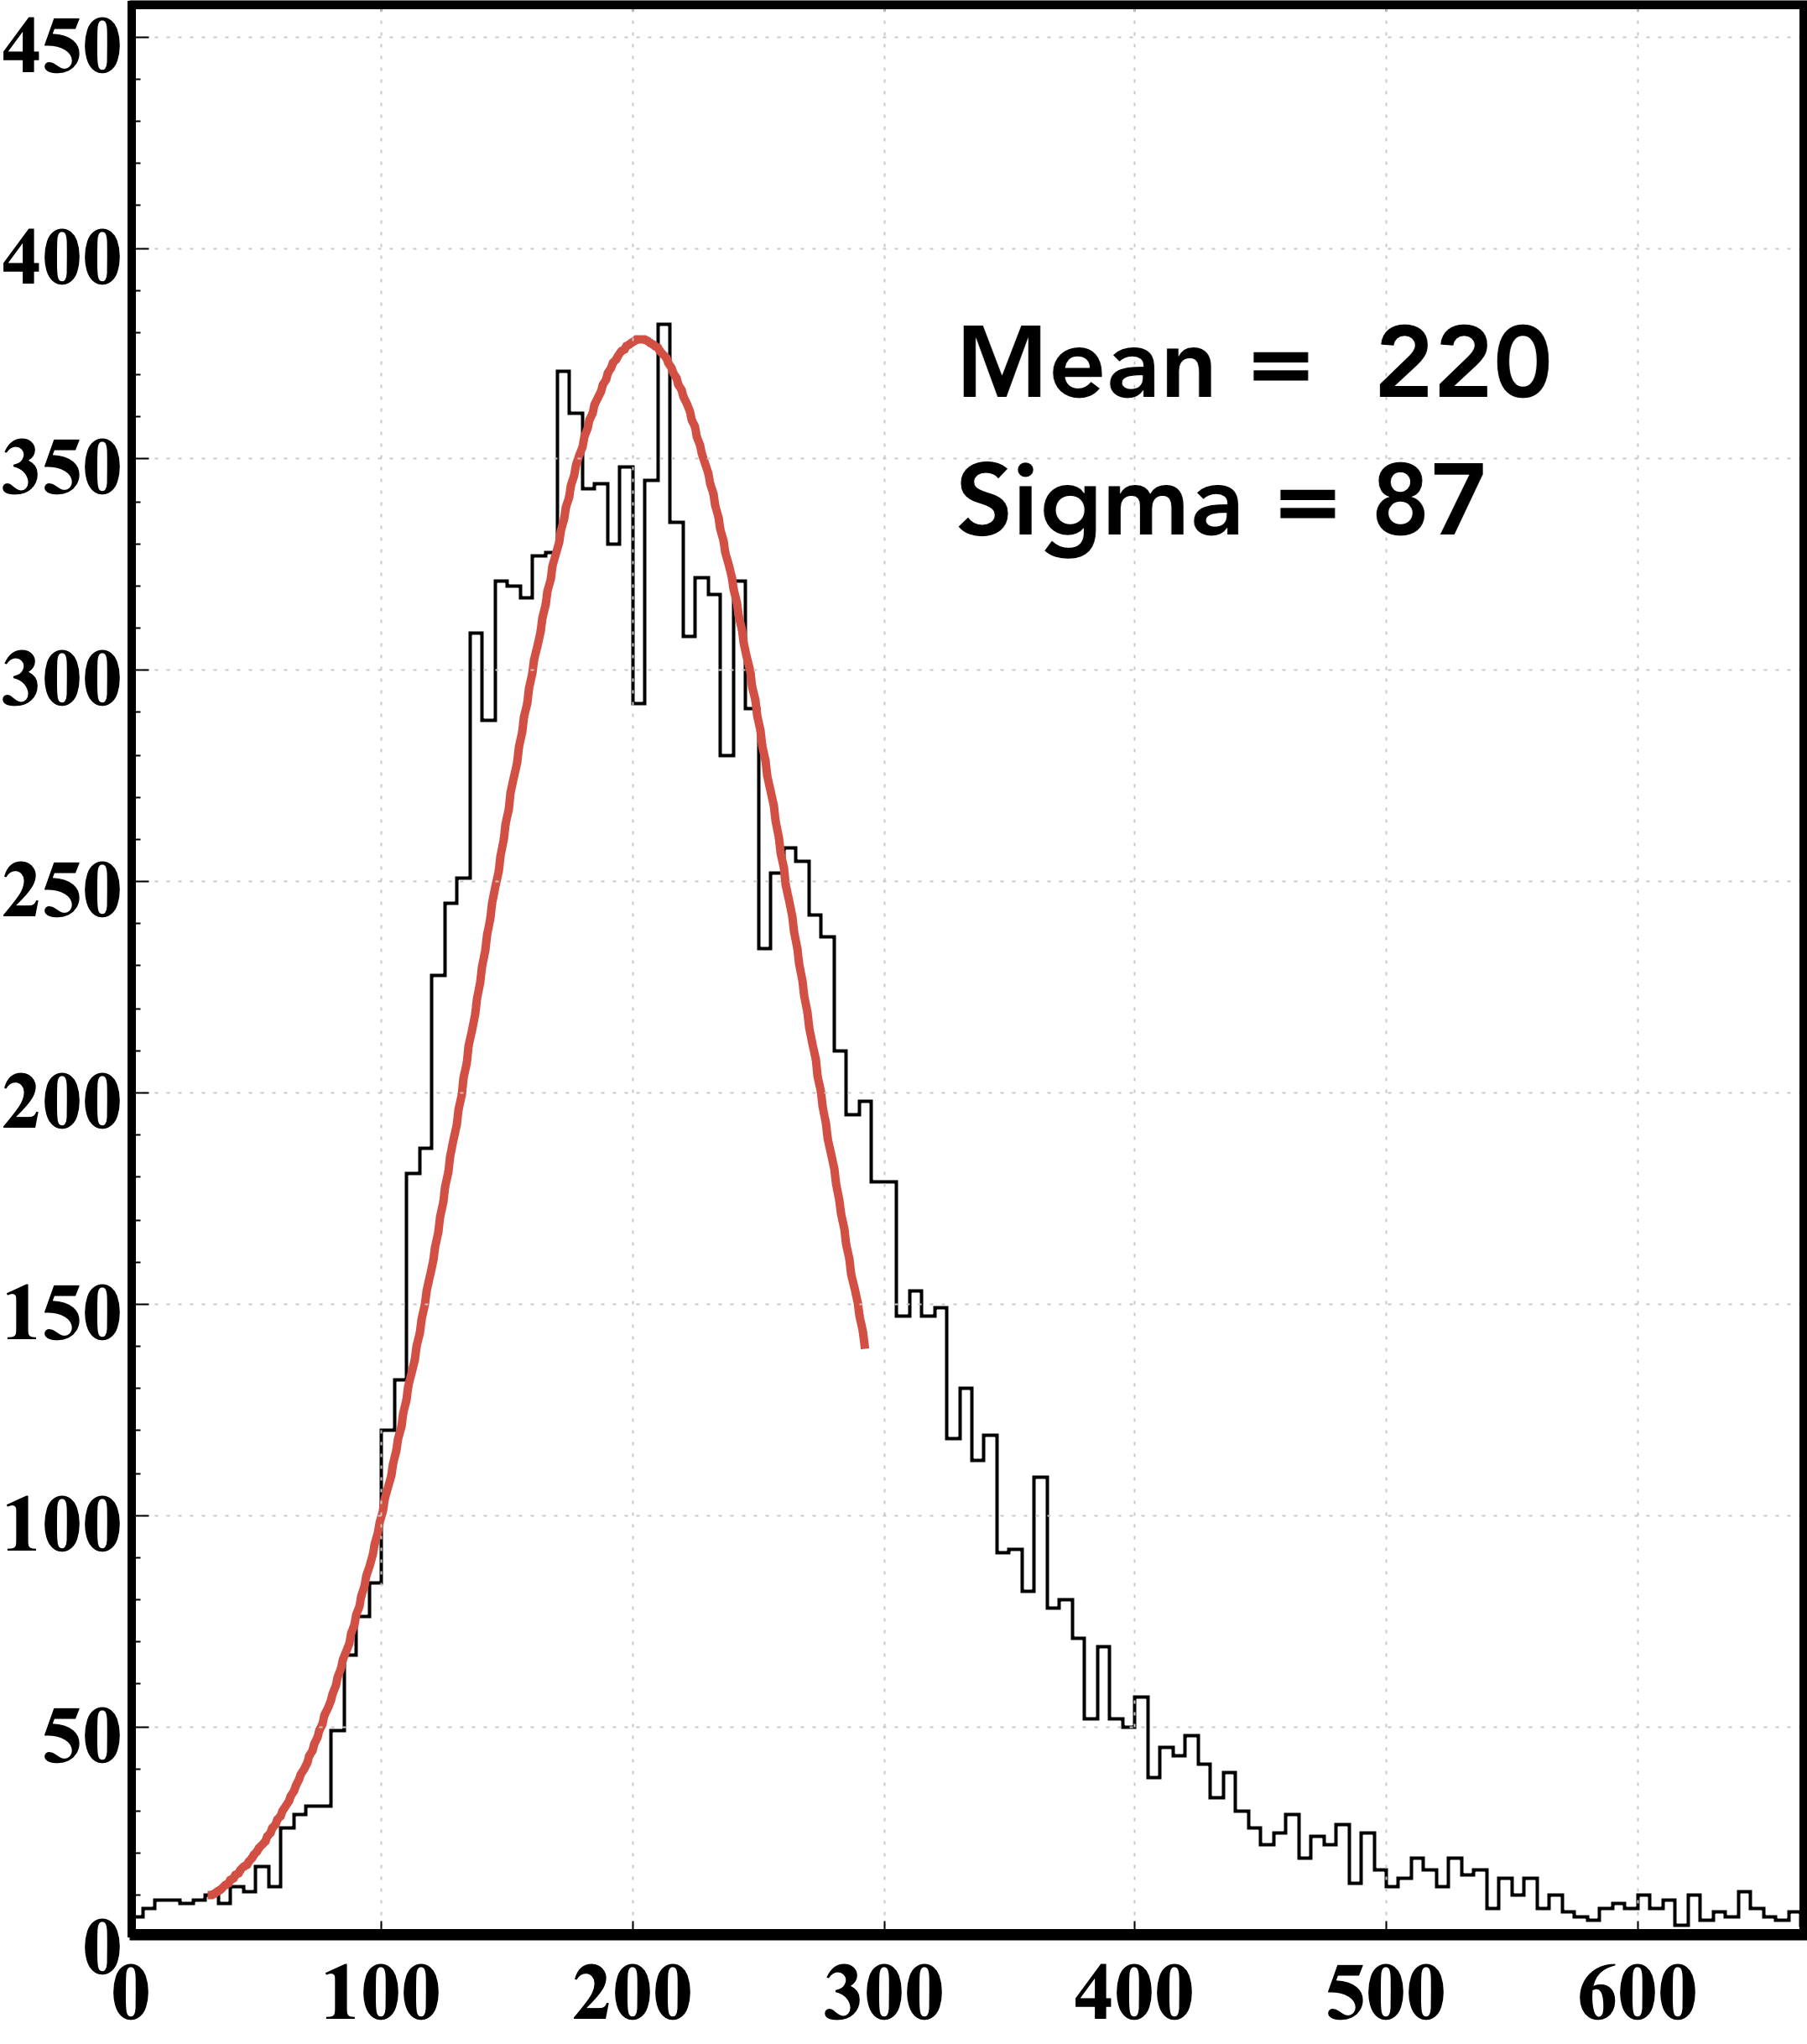
\includegraphics[width=0.47\columnwidth,height=0.75\columnwidth]{img/fadcOutput.png}
	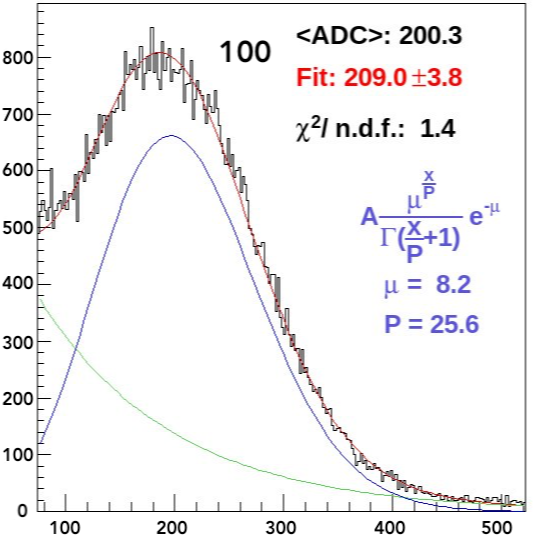
\includegraphics[width=0.47\columnwidth,height=0.75\columnwidth]{img/cc_signal.png}
	\caption{The single photoelectron FADC spectrum of one of the PMTs with the modified base (left) compared with
          the original ADC output in the configuration of a dedicated external splitter and amplifier (right). }
	\label{fig:dividerTests}
\end{figure}


